% GNUPLOT: LaTeX picture with Postscript
\begingroup
  \fontfamily{"cmr"}%
  \selectfont
  \makeatletter
  \providecommand\color[2][]{%
    \GenericError{(gnuplot) \space\space\space\@spaces}{%
      Package color not loaded in conjunction with
      terminal option `colourtext'%
    }{See the gnuplot documentation for explanation.%
    }{Either use 'blacktext' in gnuplot or load the package
      color.sty in LaTeX.}%
    \renewcommand\color[2][]{}%
  }%
  \providecommand\includegraphics[2][]{%
    \GenericError{(gnuplot) \space\space\space\@spaces}{%
      Package graphicx or graphics not loaded%
    }{See the gnuplot documentation for explanation.%
    }{The gnuplot epslatex terminal needs graphicx.sty or graphics.sty.}%
    \renewcommand\includegraphics[2][]{}%
  }%
  \providecommand\rotatebox[2]{#2}%
  \@ifundefined{ifGPcolor}{%
    \newif\ifGPcolor
    \GPcolortrue
  }{}%
  \@ifundefined{ifGPblacktext}{%
    \newif\ifGPblacktext
    \GPblacktexttrue
  }{}%
  % define a \g@addto@macro without @ in the name:
  \let\gplgaddtomacro\g@addto@macro
  % define empty templates for all commands taking text:
  \gdef\gplbacktext{}%
  \gdef\gplfronttext{}%
  \makeatother
  \ifGPblacktext
    % no textcolor at all
    \def\colorrgb#1{}%
    \def\colorgray#1{}%
  \else
    % gray or color?
    \ifGPcolor
      \def\colorrgb#1{\color[rgb]{#1}}%
      \def\colorgray#1{\color[gray]{#1}}%
      \expandafter\def\csname LTw\endcsname{\color{white}}%
      \expandafter\def\csname LTb\endcsname{\color{black}}%
      \expandafter\def\csname LTa\endcsname{\color{black}}%
      \expandafter\def\csname LT0\endcsname{\color[rgb]{1,0,0}}%
      \expandafter\def\csname LT1\endcsname{\color[rgb]{0,1,0}}%
      \expandafter\def\csname LT2\endcsname{\color[rgb]{0,0,1}}%
      \expandafter\def\csname LT3\endcsname{\color[rgb]{1,0,1}}%
      \expandafter\def\csname LT4\endcsname{\color[rgb]{0,1,1}}%
      \expandafter\def\csname LT5\endcsname{\color[rgb]{1,1,0}}%
      \expandafter\def\csname LT6\endcsname{\color[rgb]{0,0,0}}%
      \expandafter\def\csname LT7\endcsname{\color[rgb]{1,0.3,0}}%
      \expandafter\def\csname LT8\endcsname{\color[rgb]{0.5,0.5,0.5}}%
    \else
      % gray
      \def\colorrgb#1{\color{black}}%
      \def\colorgray#1{\color[gray]{#1}}%
      \expandafter\def\csname LTw\endcsname{\color{white}}%
      \expandafter\def\csname LTb\endcsname{\color{black}}%
      \expandafter\def\csname LTa\endcsname{\color{black}}%
      \expandafter\def\csname LT0\endcsname{\color{black}}%
      \expandafter\def\csname LT1\endcsname{\color{black}}%
      \expandafter\def\csname LT2\endcsname{\color{black}}%
      \expandafter\def\csname LT3\endcsname{\color{black}}%
      \expandafter\def\csname LT4\endcsname{\color{black}}%
      \expandafter\def\csname LT5\endcsname{\color{black}}%
      \expandafter\def\csname LT6\endcsname{\color{black}}%
      \expandafter\def\csname LT7\endcsname{\color{black}}%
      \expandafter\def\csname LT8\endcsname{\color{black}}%
    \fi
  \fi
  \setlength{\unitlength}{0.0500bp}%
  \begin{picture}(8640.00,6048.00)%
    \gplgaddtomacro\gplbacktext{%
      \csname LTb\endcsname%
      \put(666,576){\makebox(0,0)[r]{\strut{} 0}}%
      \csname LTb\endcsname%
      \put(666,1627){\makebox(0,0)[r]{\strut{} 0.2}}%
      \csname LTb\endcsname%
      \put(666,2678){\makebox(0,0)[r]{\strut{} 0.4}}%
      \csname LTb\endcsname%
      \put(666,3729){\makebox(0,0)[r]{\strut{} 0.6}}%
      \csname LTb\endcsname%
      \put(666,4780){\makebox(0,0)[r]{\strut{} 0.8}}%
      \csname LTb\endcsname%
      \put(666,5831){\makebox(0,0)[r]{\strut{} 1}}%
      \csname LTb\endcsname%
      \put(774,396){\makebox(0,0){\strut{} 2}}%
      \csname LTb\endcsname%
      \put(2282,396){\makebox(0,0){\strut{} 4}}%
      \csname LTb\endcsname%
      \put(3790,396){\makebox(0,0){\strut{} 6}}%
      \csname LTb\endcsname%
      \put(5298,396){\makebox(0,0){\strut{} 8}}%
      \csname LTb\endcsname%
      \put(6806,396){\makebox(0,0){\strut{} 10}}%
      \csname LTb\endcsname%
      \put(8314,396){\makebox(0,0){\strut{} 12}}%
      \put(144,3203){\rotatebox{-270}{\makebox(0,0){\strut{}CDF}}}%
      \put(4544,126){\makebox(0,0){\strut{}Achievable rate ${R}$ [bit/s/Hz]}}%
      \put(5298,4255){\makebox(0,0)[l]{\strut{}\framebox{$t=2\quad r=2$\quad SNR=15\,dB}}}%
    }%
    \gplgaddtomacro\gplfronttext{%
      \csname LTb\endcsname%
      \put(7495,2223){\makebox(0,0)[r]{\strut{}$M=2$ simul.}}%
      \csname LTb\endcsname%
      \put(7495,1935){\makebox(0,0)[r]{\strut{}$M=2$ Gamma}}%
      \csname LTb\endcsname%
      \put(7495,1647){\makebox(0,0)[r]{\strut{}$M=4$ simul.}}%
      \csname LTb\endcsname%
      \put(7495,1359){\makebox(0,0)[r]{\strut{}$M=4$ Gamma}}%
      \csname LTb\endcsname%
      \put(7495,1071){\makebox(0,0)[r]{\strut{}$M=8$ simul.}}%
      \csname LTb\endcsname%
      \put(7495,783){\makebox(0,0)[r]{\strut{}$M=8$ Gamma}}%
    }%
    \gplbacktext
    \put(0,0){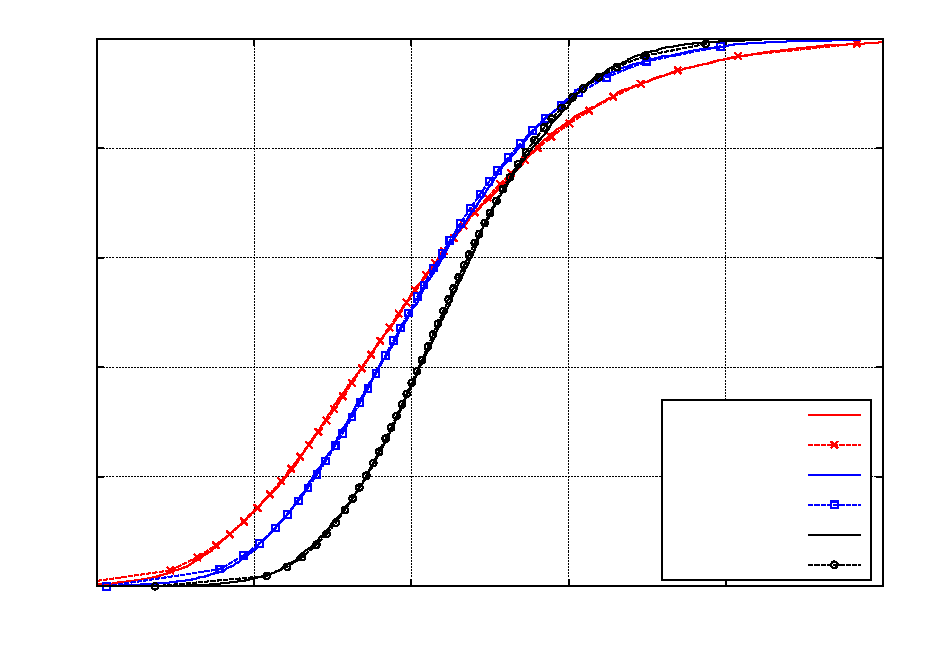
\includegraphics{CDFgamma}}%
    \gplfronttext
  \end{picture}%
\endgroup
